\documentclass[11pt, letterpaper]{article}
\usepackage[margin=1in]{geometry}
\usepackage{graphicx}
\usepackage{booktabs}
\usepackage{caption}
\usepackage{subcaption}
\usepackage{hyperref}
\usepackage{parskip}
\usepackage{array}
\usepackage{tabularx}
\usepackage{amsmath}
\usepackage{amssymb}
\usepackage{float}

\captionsetup{font=small, labelfont=bf, width=0.92\textwidth}

\title{\textbf{Homework 4: Streamflow Prediction with Sequence Models}}
\author{Nabin Kalauni}
\date{HWRS 640 --- Spring 2026}

\begin{document}
\maketitle

% ─────────────────────────────────────────────────────────────────────────────
\section{Problem 1: Data Access and Exploratory Analysis}
% ─────────────────────────────────────────────────────────────────────────────

The code for this assignment is available in the GitHub repository:
\url{https://github.com/nkalauni/hwrs640_rnn_hw}.

\subsection{Dataset Overview}

The miniCAMELS dataset was accessed via the \texttt{MiniCamels} Python package.
Table~\ref{tab:dataset} summarizes the key dataset properties.

\begin{table}[H]
    \centering
    \caption{miniCAMELS dataset summary.}
    \label{tab:dataset}
    \begin{tabular}{ll}
        \toprule
        Property & Value \\
        \midrule
        Number of basins         & 50 \\
        Period                   & WY1981--WY2010 (Oct 1980 -- Sep 2010) \\
        Dynamic input variables  & \texttt{prcp}, \texttt{tmax}, \texttt{tmin}, \texttt{srad}, \texttt{vp} (5 vars) \\
        Target variable          & \texttt{qobs} (mm/day) \\
        Static attributes        & 16 (aridity, LAI, baseflow index, forest fraction, etc.) \\
        Total input features     & 21 (5 dynamic + 16 static, per timestep) \\
        \bottomrule
    \end{tabular}
\end{table}

\subsection{Train/Validation/Test Split}

A strictly temporal split was applied uniformly across all 50 basins:

\begin{itemize}
    \item \textbf{Train:} WY1981--WY2003 (Oct 1, 1980 -- Sep 30, 2003; 23 years)
    \item \textbf{Validation:} WY2004--WY2006 (Oct 1, 2003 -- Sep 30, 2006; 3 years)
    \item \textbf{Test:} WY2007--WY2010 (Oct 1, 2006 -- Sep 30, 2010; 4 years)
\end{itemize}

A temporal hold-out is the standard approach in catchment hydrology because it
evaluates true out-of-sample temporal generalization, matching the operational
use case of predicting future streamflow from future forcings.  Holding out a
contiguous future block prevents any lookahead leakage: no future observation
can influence a training-set statistic or normalization parameter.  Splitting
by basin is also a valid approach to recreate a Prediction in Ungauged Basins
(PUB) scneario. However, with only 50 basins, a spatial split would reduce the 
training data too much so we chose a temporal split.

\subsection{Supervised Learning Sample Construction}

Each sample consists of a 365-day sliding window of meteorological forcings
paired with a single streamflow prediction target:

\begin{itemize}
    \item \textbf{Input:} $\mathbf{X} \in \mathbb{R}^{365 \times 21}$ --- 365
          days of 5 Daymet forcings, with the 16 static basin attributes tiled
          along the time dimension so the model sees them at every timestep.
    \item \textbf{Target:} \texttt{qobs} at the final timestep of the window
          (one-step-ahead prediction of streamflow for day $t$ given forcings
          and antecedent conditions from days $t-364$ through $t$).
\end{itemize}

A 365-day window was chosen to capture a full annual hydrological cycle,
including seasonal snowmelt signals and inter-annual variability in antecedent
soil moisture, which are important for accurate streamflow prediction.

\subsection{Exploratory Data Analysis}

Figure~\ref{fig:eda_hist} shows the distribution of observed daily streamflow
across all basins and all three splits.  The distribution is strongly
right-skewed: the vast majority of days have low streamflow, but extreme flood
events can exceed 10--100$\times$ the median.  This motivates z-score
normalization of \texttt{qobs} before training rather than raw values.

Figure~\ref{fig:eda_ts} shows daily streamflow time series for five example
basins spanning the full 30-year record.  The basins exhibit markedly different
hydrological regimes: some show sharp spring snowmelt peaks, others show
flashy summer convective responses, and still others have more subdued
perennial baseflow.  This diversity tests the model's ability to generalize
across climatic gradients.

\begin{figure}[H]
    \centering
    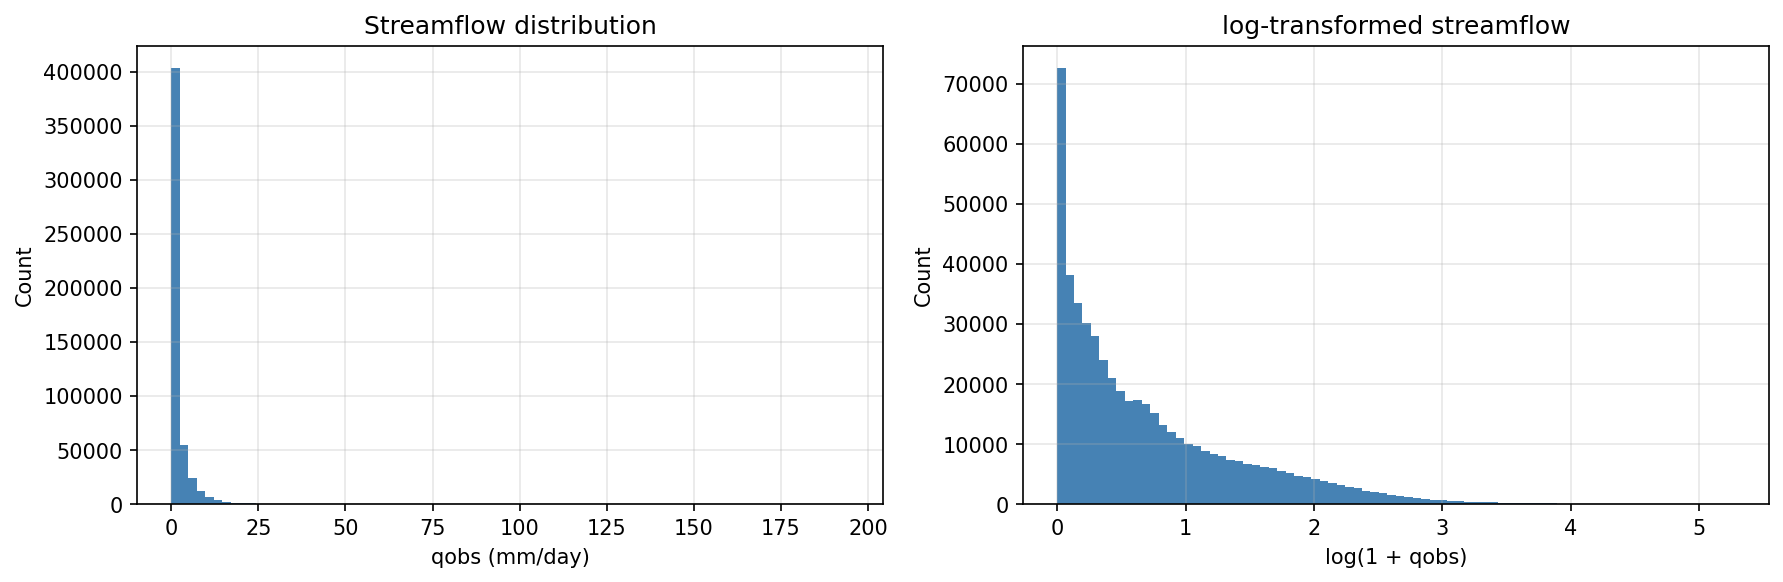
\includegraphics[width=0.78\textwidth]{outputs/eda/qobs_histogram.png}
    \caption{Distribution of observed daily streamflow (\texttt{qobs}, mm/day) pooled
    across all 50 basins. The strong right skew motivates z-score normalization
    prior to model training.}
    \label{fig:eda_hist}
\end{figure}

\begin{figure}[H]
    \centering
    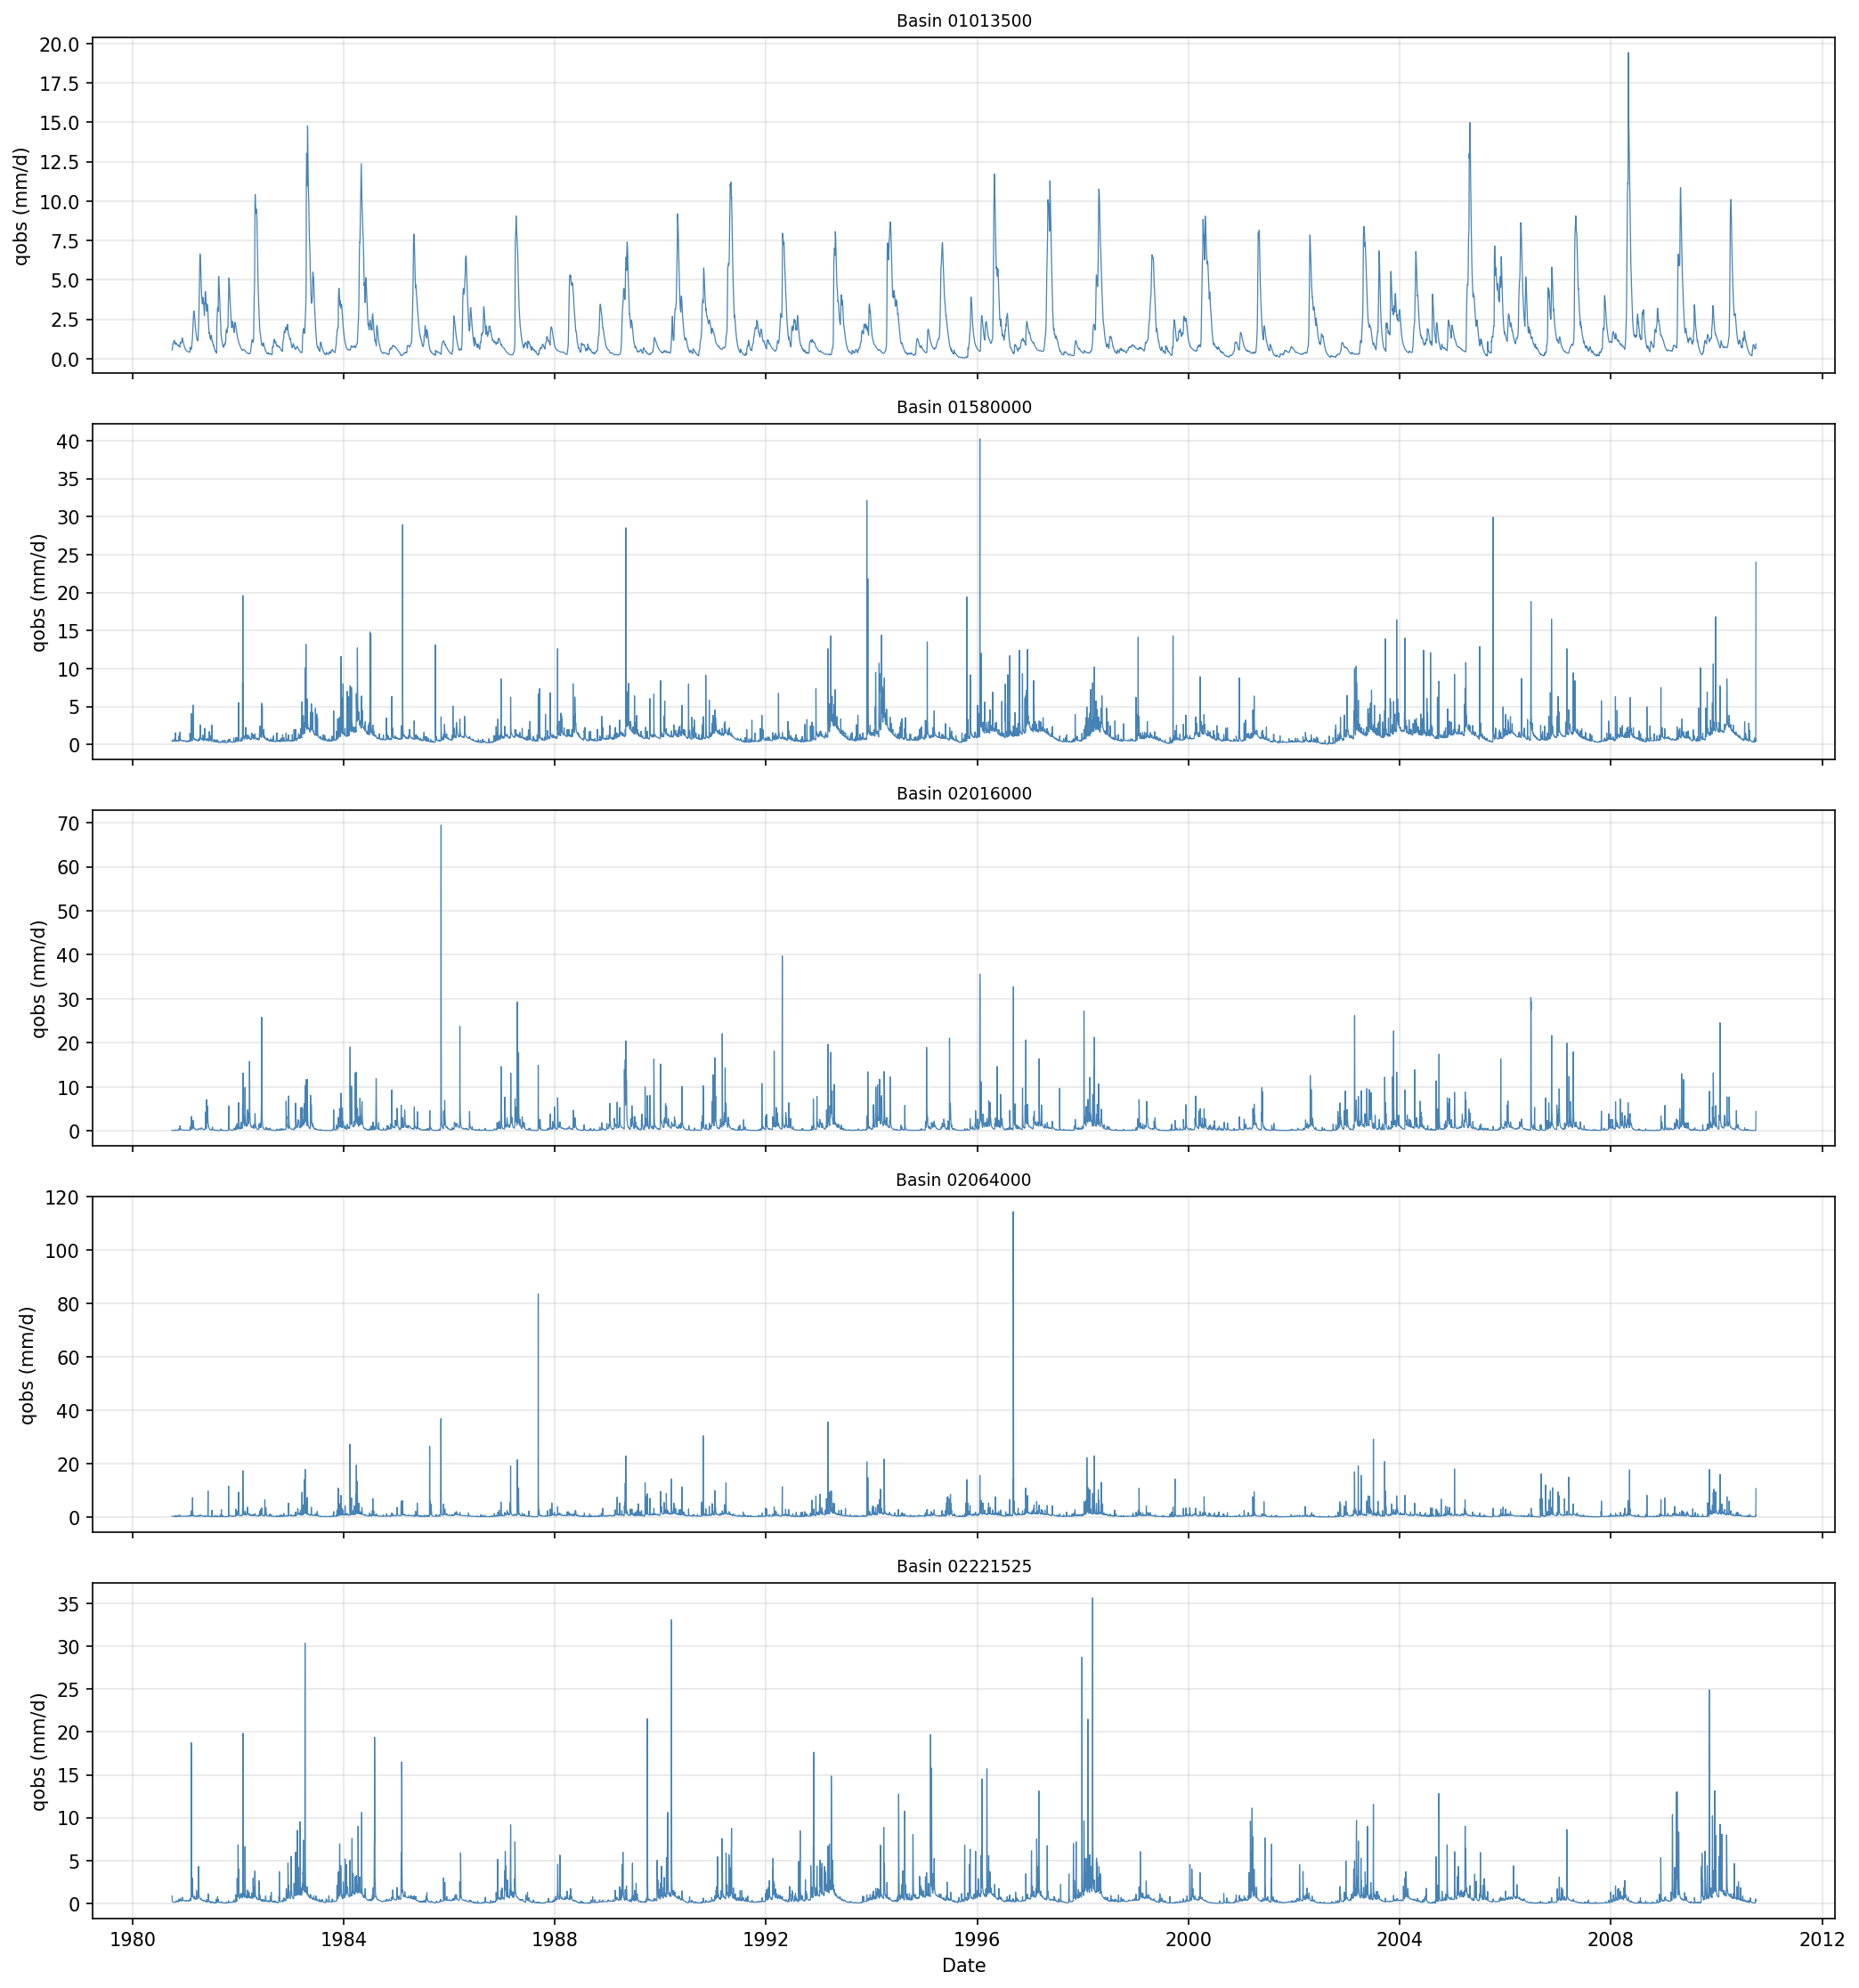
\includegraphics[width=\textwidth]{outputs/eda/streamflow_timeseries.png}
    \caption{Daily streamflow time series for five example miniCAMELS basins
    (WY1981--WY2010). Vertical dashed lines mark the train/val and val/test
    boundaries. Basins display diverse regimes ranging from nival to flashy
    pluvial.}
    \label{fig:eda_ts}
\end{figure}

\subsection{Preprocessing}

\textbf{Missing values:} Rows with missing \texttt{qobs} were dropped before
window construction.  Dynamic forcings had no missing values in the dataset.

\textbf{Normalization:} All dynamic features, \texttt{qobs}, and static
attributes were z-score normalized ($\mu$, $\sigma$ computed on the training
split only) and stored as pickled \texttt{Normalizer} objects for reproducible
evaluation.  Predictions are inverse-transformed before metric computation.

\textbf{Static attributes:} The 16 static attributes (one vector per basin)
were normalized using training-basin statistics and tiled along the time axis
so that each timestep of the input sequence carries both dynamic and static
information.  This simple concatenation approach avoids a separate static
encoder while still injecting catchment characteristics. But it does mean more data
redundancy and a larger input dimension for the sequence model to process.

\textbf{Sequence windows:} Overlapping 365-day sliding windows were extracted
from each basin's time series within each split.  This produces approximately
$50 \times 8{,}400 \approx 420{,}000$ training samples, $50 \times 1{,}100 \approx 55{,}000$
validation samples, and $50 \times 1{,}450 \approx 72{,}500$ test samples.

% ─────────────────────────────────────────────────────────────────────────────
\section{Problem 2: Model Design}
% ─────────────────────────────────────────────────────────────────────────────

Two sequence model architectures were implemented and compared.

\subsection{LSTM}

The LSTM model is a two-layer stacked LSTM followed by a linear output head:

\begin{enumerate}
    \item \textbf{Input:} $\mathbf{X} \in \mathbb{R}^{B \times 365 \times 21}$
    \item \textbf{Layer 1:} LSTM ($\text{input}=21$, $\text{hidden}=128$, $\text{dropout}=0.2$)
    \item \textbf{Layer 2:} LSTM ($\text{input}=128$, $\text{hidden}=128$, $\text{dropout}=0.2$)
    \item \textbf{Head:} Dropout(0.2) $\rightarrow$ Linear($128 \rightarrow 1$)
    \item \textbf{Read-out:} Last hidden state $\mathbf{h}_{T}$ at $t=365$.
\end{enumerate}

\noindent Total trainable parameters: \textbf{208,513}.

Static attributes enter the model by being concatenated to each timestep of the
dynamic input sequence, so the LSTM processes 21 features per step rather than 5.

\textbf{Appropriateness for streamflow:} LSTMs were first applied to
rainfall-runoff by Kratzert et al.\ (2018) and have since become a benchmark.
The gated recurrent structure acts as a learned conceptual store, naturally
simulating the role of soil moisture, groundwater, and snowpack.

\textbf{Strength:} Handles long-range dependencies and captures seasonality through
selective forgetting; well-studied for hydrology.

\textbf{Weakness:} Sequential computation cannot be parallelized over the time
dimension; a fixed-size hidden state may compress information as the sequence
length grows.

\subsection{Transformer}

The Transformer model uses a linear embedding layer, sinusoidal positional
encoding, and a stack of two pre-norm TransformerEncoder layers, followed by
mean-pooling and a linear output head:

\begin{enumerate}
    \item \textbf{Input projection:} Linear($21 \rightarrow 128$)
    \item \textbf{Positional encoding:} Sinusoidal (Vaswani et al., 2017)
    \item \textbf{Encoder $\times$2:} TransformerEncoderLayer
          ($d_\text{model}=128$, $n_\text{head}=4$, $d_\text{ff}=256$,
          $\text{dropout}=0.2$, pre-norm)
    \item \textbf{Pooling:} Mean over the time dimension
    \item \textbf{Head:} Dropout(0.2) $\rightarrow$ Linear($128 \rightarrow 1$)
\end{enumerate}

\noindent Total trainable parameters: \textbf{267,905}.

Static attributes are injected the same way as for the LSTM.

\textbf{Appropriateness:} The self-attention mechanism can in principle attend
to arbitrary lag relationships without distance decay, which could be
advantageous for capturing remote snowmelt or monsoon precursors.

\textbf{Strength:} Fully parallel training; attention can explicitly link
precipitation events to delayed flow responses anywhere in the 365-day context.

\textbf{Weakness:} Attention complexity is $O(T^2)$ in sequence length;
with only 50 basins the Transformer may lack the data needed to learn
meaningful attention patterns compared to the LSTM's stronger inductive bias
toward sequential dynamics.

% ─────────────────────────────────────────────────────────────────────────────
\section{Problem 3: Training Pipeline}
% ─────────────────────────────────────────────────────────────────────────────

\subsection{Training Configuration}

Both models were trained with the same hyperparameter configuration, summarized
in Table~\ref{tab:training}.  The CLI exposes all of these as command-line
arguments (e.g., \texttt{--lr}, \texttt{--epochs}, \texttt{--hidden-size}).

\begin{table}[H]
    \centering
    \caption{Training hyperparameters shared by both models.}
    \label{tab:training}
    \begin{tabular}{ll}
        \toprule
        Hyperparameter & Value \\
        \midrule
        Sequence length     & 365 days \\
        Batch size          & 256 \\
        Optimizer           & Adam \\
        Learning rate       & $1\times10^{-3}$ \\
        Loss function       & MSE (normalized space) \\
        Max epochs          & 30 \\
        Early stopping      & patience = 10 epochs (best val loss) \\
        Dropout             & 0.2 \\
        Hidden size / $d_\text{model}$ & 128 \\
        Number of layers    & 2 \\
        Random seed         & 42 \\
        \bottomrule
    \end{tabular}
\end{table}

The LSTM converged in \textbf{23 epochs} (best validation NSE = 0.889);
the Transformer ran the full \textbf{32 epochs} before early stopping
(best validation NSE = 0.836).

\subsection{Training Curves}

Figure~\ref{fig:training_curves} shows training and validation loss curves
and validation NSE for both models.  The LSTM converges smoothly and reaches
a lower validation loss, with validation NSE climbing steadily to $\approx$0.89.
The Transformer converges more slowly with greater epoch-to-epoch variability in
validation loss, reflecting the architecture's weaker inductive bias for
sequential data.

\begin{figure}[H]
    \centering
    \begin{subfigure}[b]{0.49\textwidth}
        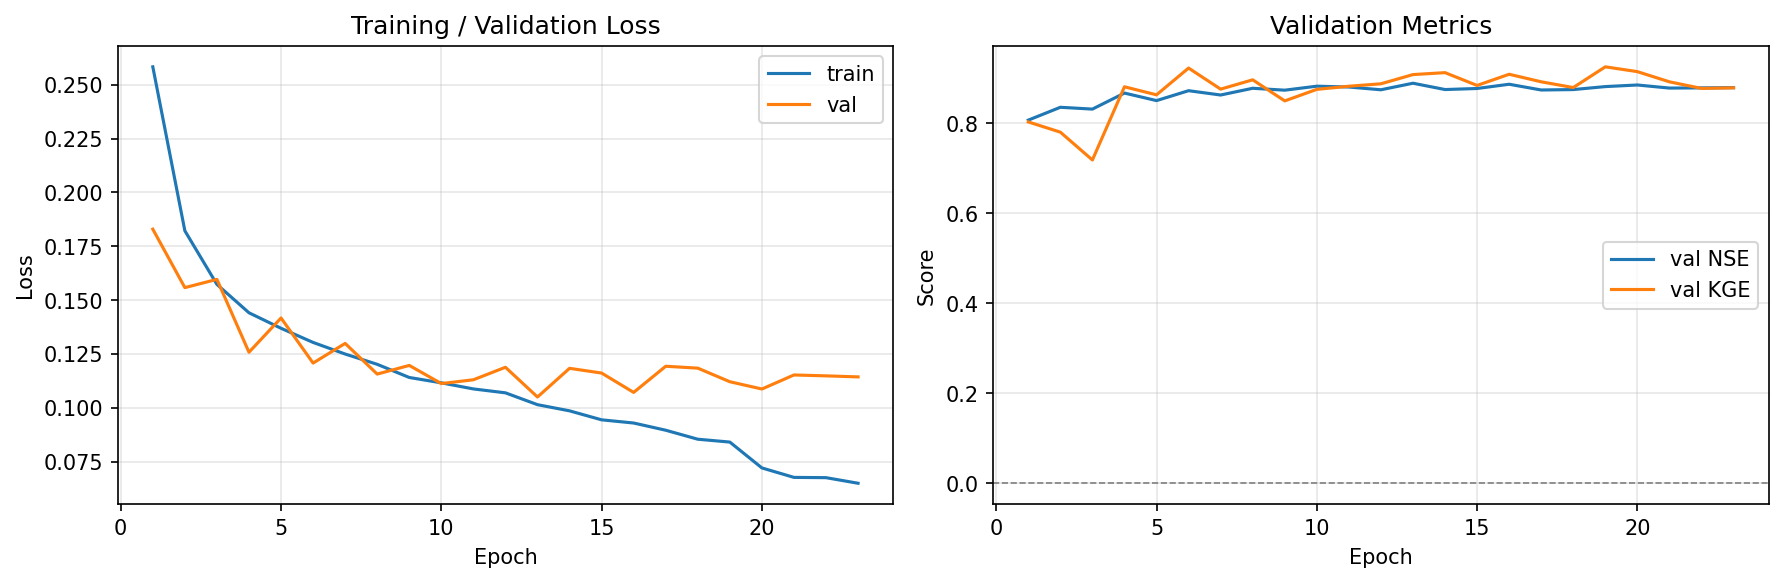
\includegraphics[width=\textwidth]{outputs/plots/lstm/lstm_training_curves.png}
        \caption{LSTM (23 epochs, best val NSE = 0.889)}
    \end{subfigure}
    \hfill
    \begin{subfigure}[b]{0.49\textwidth}
        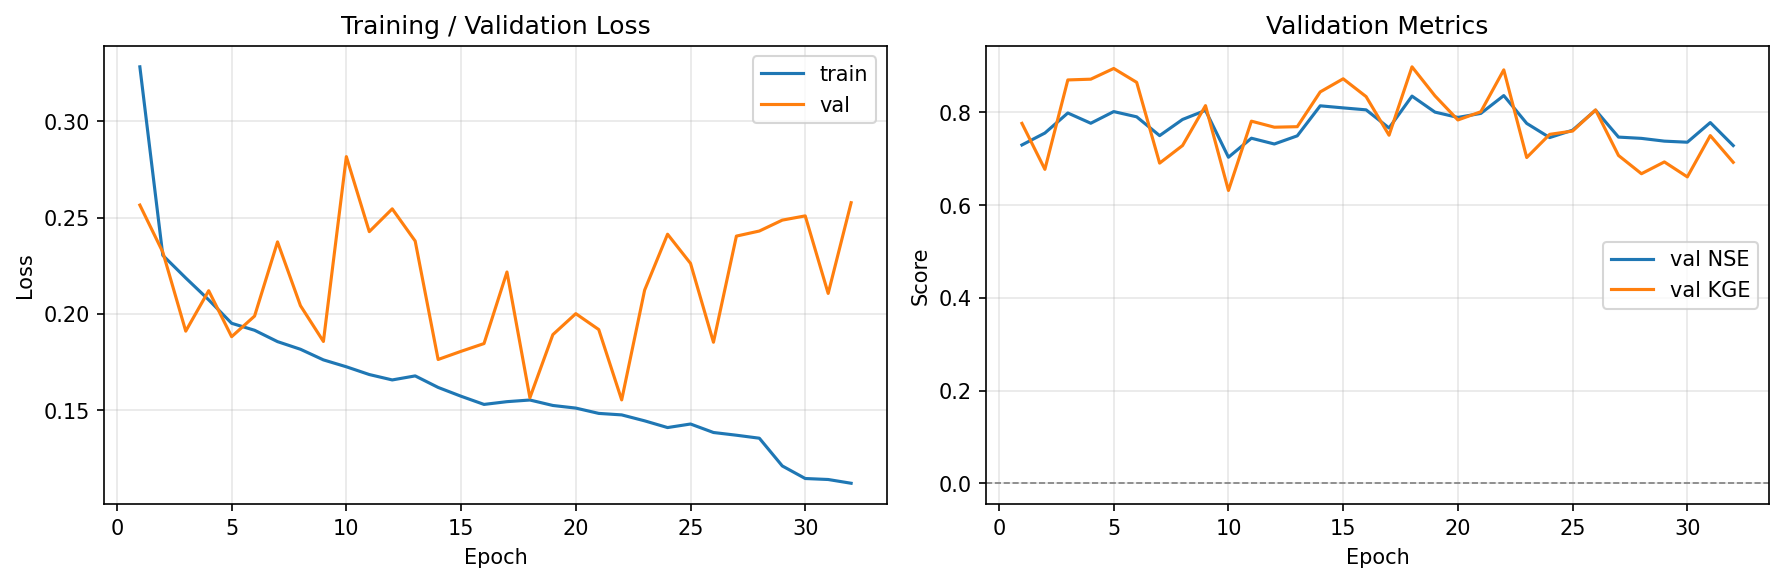
\includegraphics[width=\textwidth]{outputs/plots/transformer/transformer_training_curves.png}
        \caption{Transformer (32 epochs, best val NSE = 0.836)}
    \end{subfigure}
    \caption{Training and validation loss and NSE curves for both models.
    The LSTM converges faster and achieves a higher peak validation NSE.}
    \label{fig:training_curves}
\end{figure}

% ─────────────────────────────────────────────────────────────────────────────
\section{Problem 4: Evaluation and Interpretation}
% ─────────────────────────────────────────────────────────────────────────────

\subsection{Test-Set Metrics}

Both models were evaluated on the held-out test set (WY2007--WY2010) across
all 50 basins.  Table~\ref{tab:metrics} reports the median of each metric.
The LSTM substantially outperforms the Transformer on every metric.

\begin{table}[H]
    \centering
    \caption{Test-set performance (median across 50 basins). PBIAS is reported
    as the median of the absolute value.}
    \label{tab:metrics}
    \begin{tabular}{lrrrrr}
        \toprule
        Model & NSE $\uparrow$ & KGE $\uparrow$ & RMSE $\downarrow$ & MAE $\downarrow$ & |PBIAS| $\downarrow$ \\
        \midrule
        LSTM        & \textbf{0.778} & \textbf{0.774} & \textbf{0.909} & \textbf{0.420} & \textbf{13.1\%} \\
        Transformer & 0.560          & 0.603          & 1.508          & 0.689          & 18.2\% \\
        \bottomrule
    \end{tabular}
\end{table}

The LSTM achieves NSE $> 0.5$ (``satisfactory'' by Moriasi et al.\ 2007
guidelines) for \textbf{84\%} of basins and NSE $> 0.7$ for \textbf{62\%}.
The Transformer achieves NSE $> 0.5$ for only \textbf{58\%} of basins and
NSE $> 0.7$ for just \textbf{20\%}, underscoring the large performance gap.

Figure~\ref{fig:cdf} visualizes the full empirical CDFs of all five metrics.
The LSTM CDF is consistently shifted toward better values across every metric.

\begin{figure}[H]
    \centering
    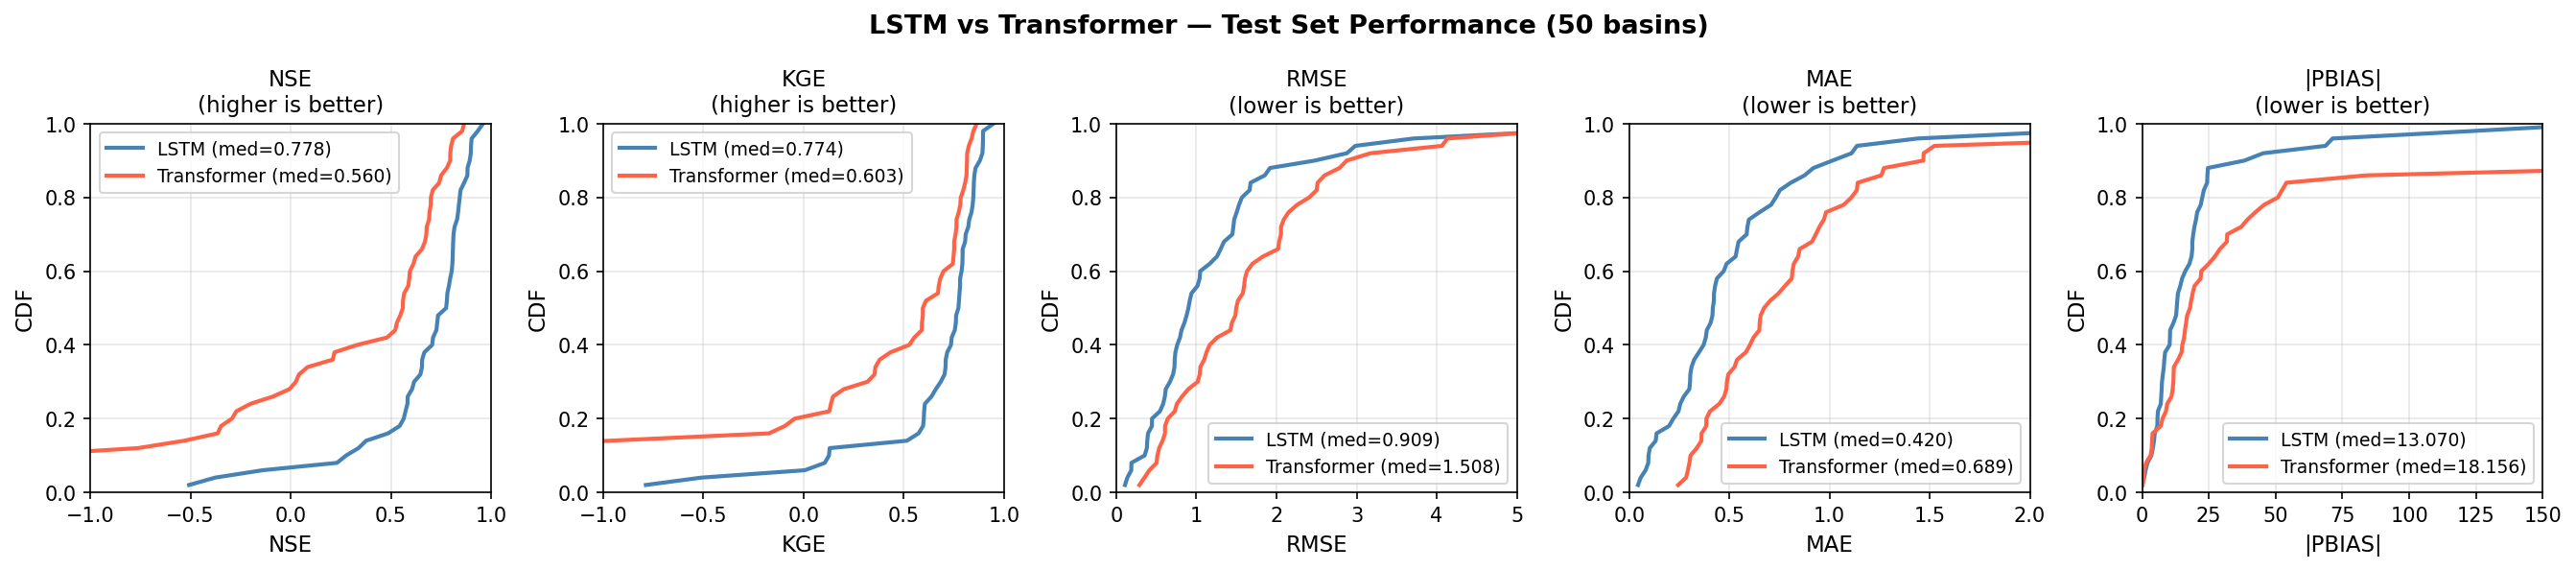
\includegraphics[width=\textwidth]{outputs/plots/comparison_cdf.png}
    \caption{Empirical CDFs of test-set performance metrics for the LSTM
    (blue) and Transformer (red) across all 50 basins.  Median values are
    shown in the legend.  PBIAS is the absolute value; x-axes are clipped
    to highlight the central distribution.}
    \label{fig:cdf}
\end{figure}

\subsection{Best-Performing Basin (LSTM): 12358500}

Basin \texttt{12358500} achieved the highest LSTM test NSE of \textbf{0.960}
(KGE = 0.895, PBIAS = $+8.6\%$).  This basin is located in the Pacific
Northwest (northern Rockies / Cascades region), a snowmelt-dominated
catchment with a pronounced and predictable spring runoff peak.  The strongly
seasonal, single-peaked hydrograph provides clear temporal structure that the
LSTM's gated recurrence can exploit: the forget gate learns to retain
snowpack accumulation signals over winter while the input gate activates
during the spring melt period.  Figure~\ref{fig:best} shows close agreement
between simulated and observed hydrographs throughout the test period, with
the model accurately capturing both the timing and magnitude of peak flows.

\begin{figure}[H]
    \centering
    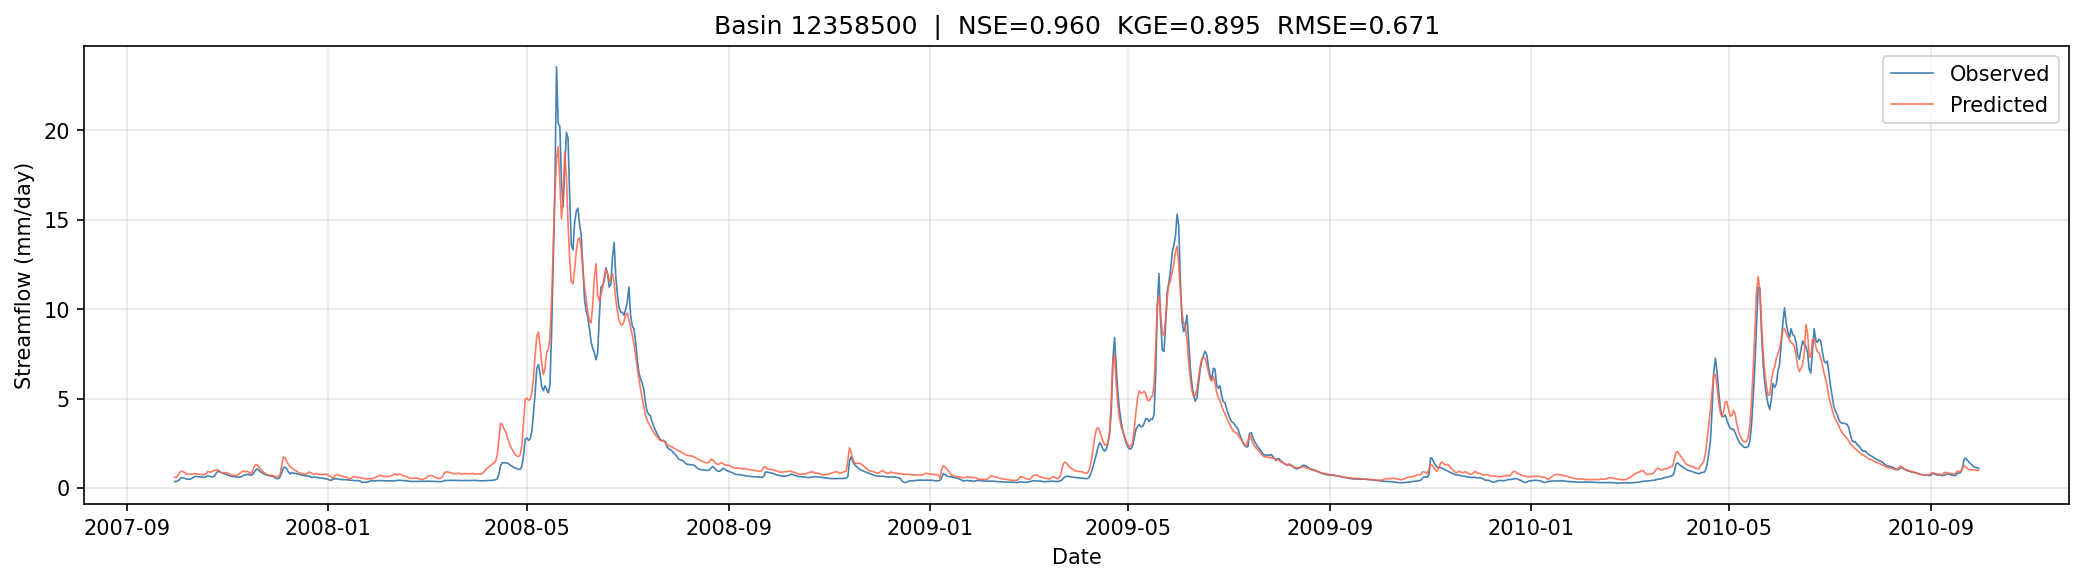
\includegraphics[width=\textwidth]{outputs/plots/lstm/lstm_hydrograph_best_12358500.png}
    \caption{LSTM hydrograph for best basin (12358500, NSE = 0.960).
    Observed (blue) and simulated (orange) daily streamflow over the
    WY2007--WY2010 test period.}
    \label{fig:best}
\end{figure}

\subsection{Worst-Performing Basin (LSTM): 02297310}

Basin \texttt{02297310} had the worst LSTM test NSE of \textbf{$-$0.507}
(KGE $\approx$ 0.006, PBIAS = $+69\%$).  This basin is located in the
low-gradient coastal plain of Florida and is characterized by
groundwater-dominated, flashy streamflow with a weak or absent seasonal
signal.  The positive bias indicates systematic overestimation: the model
likely generalizes the precipitation-driven runoff dynamics it learned from
energy-limited basins in the training set, while failing to account for
the highly permeable soils and rapid subsurface drainage typical of this
karst-influenced region.  Lacking explicit soil or geology information
beyond what is encoded in the 16 static attributes, the model cannot
distinguish this basin's behavior from a more typical rainfall-runoff regime.
Figure~\ref{fig:worst} illustrates the poor correspondence, with
simulated peaks greatly exceeding the relatively muted observed response.

\begin{figure}[H]
    \centering
    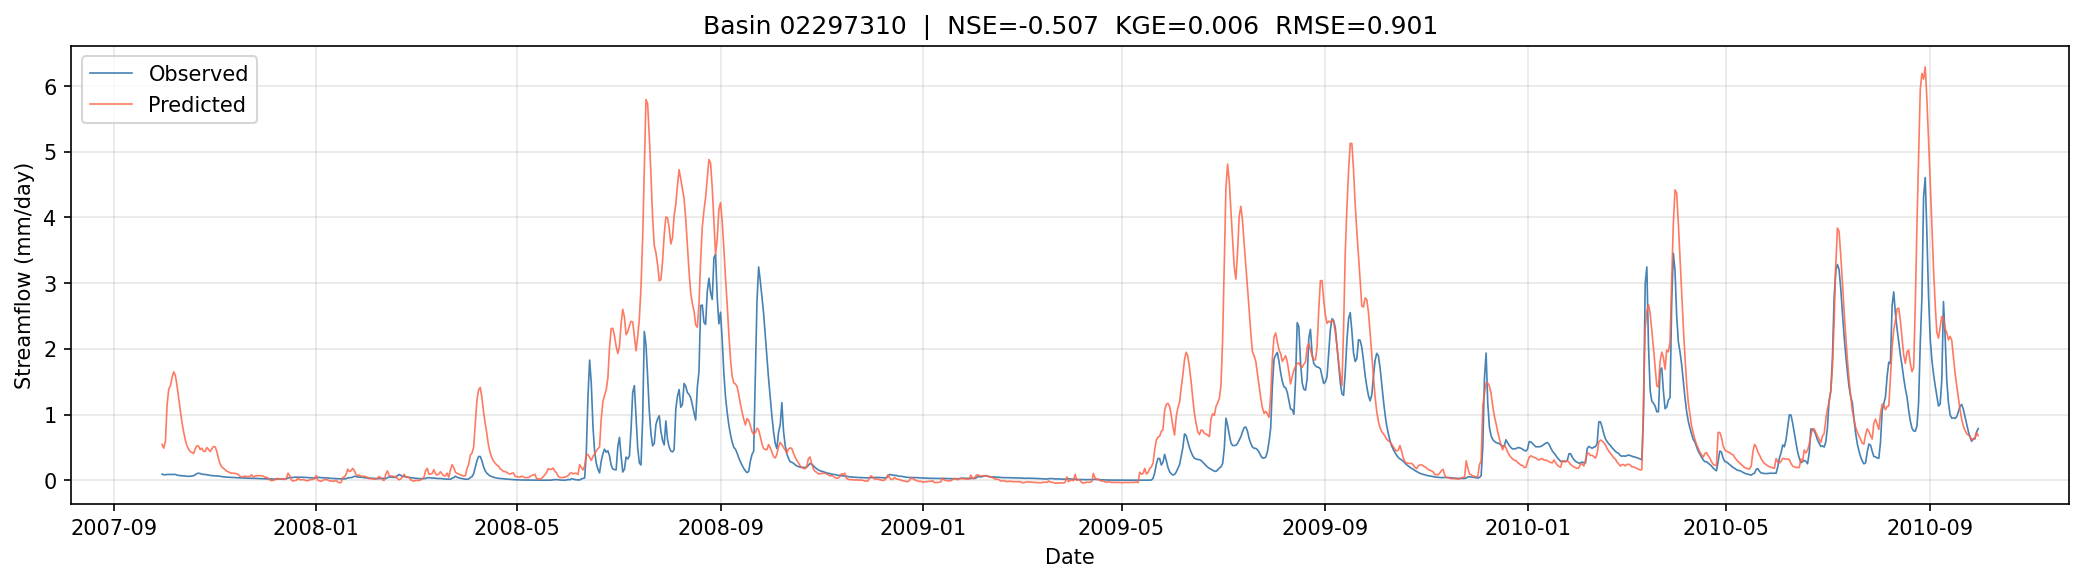
\includegraphics[width=\textwidth]{outputs/plots/lstm/lstm_hydrograph_worst_02297310.png}
    \caption{LSTM hydrograph for worst basin (02297310, NSE = $-$0.507).
    The model systematically overestimates streamflow, suggesting it fails
    to represent the unique groundwater-dominated regime of this coastal-plain
    basin.}
    \label{fig:worst}
\end{figure}

\subsection{Why the LSTM Outperforms the Transformer}

The LSTM's advantage can be attributed to three factors:

\begin{enumerate}
    \item \textbf{Inductive bias:} The recurrent gated structure of an LSTM
          is a natural fit for the sequential memory processes (soil moisture
          routing, snowpack accumulation/melt) that govern rainfall-runoff.
          This prior structure reduces the amount of data needed to learn a
          useful representation.  The Transformer, by contrast, must learn
          the relevance of temporal ordering entirely from scratch via
          positional encodings and attention patterns.

    \item \textbf{Data scale:} With only 50 basins and 23 training years,
          the dataset is relatively small for a Transformer, which typically
          requires large data volumes to train its attention heads to produce
          physically meaningful lag structures.  Several basins with atypical
          hydrology (e.g., semi-arid intermittent streams) appear to confuse
          the Transformer badly, as evidenced by catastrophic NSE values
          (basin \texttt{07148400}: NSE = $-$6.3, PBIAS = $-$417\%) that
          suggest near-random predictions.

    \item \textbf{Optimization stability:} The noisier validation loss
          curves of the Transformer (Figure~\ref{fig:training_curves}) indicate
          a harder optimization landscape with the given learning rate and
          batch size.  Transformer models often benefit from warmup schedules
          and larger batch sizes that were not explored here.
\end{enumerate}

% ─────────────────────────────────────────────────────────────────────────────
\section{Conclusion}
% ─────────────────────────────────────────────────────────────────────────────

This assignment implemented a reproducible CLI-based rainfall-runoff
prediction system using the miniCAMELS dataset.  Two sequence architectures
were trained and evaluated on 50 basins:

\begin{itemize}
    \item The \textbf{LSTM} produced strong results (median test NSE = 0.778,
          KGE = 0.774), consistent with its well-established role as a
          benchmark model in data-driven hydrology.  The model performed
          particularly well in snowmelt-dominated basins with clear seasonal
          structure and struggled most with flat, groundwater-dominated
          coastal-plain basins where its learned runoff relationships
          did not transfer.

    \item The \textbf{Transformer} underperformed substantially (median test
          NSE = 0.560), with several basins showing catastrophic failure.
          This is likely attributable to limited training data and the lack
          of the recurrent inductive bias that makes LSTMs well-suited to
          hydrological time series.  Future work could explore larger datasets,
          learning rate warmup, or hybrid architectures that combine attention
          with recurrence.
\end{itemize}

The key lesson is that architectural inductive biases matter significantly
at data scales typical in catchment hydrology: the LSTM's built-in assumption
of temporal ordering and memory provides a meaningful advantage over the
more general Transformer when training data are limited.

The code for this assignment is available in the GitHub repository:
\url{https://github.com/nkalauni/hwrs640_rnn_hw}.

\end{document}
